\documentclass[a4paper, titlepage]{article}

% For equations
\usepackage{amsmath}

% For including figures
\usepackage{graphicx}
\usepackage{float}

% Bibiliography setup
\usepackage[square]{natbib}
\bibliographystyle{agsm}
\usepackage[nottoc]{tocbibind}

% For typesetting matlab
\usepackage{listings}
\usepackage{color} %red, green, blue, yellow, cyan, magenta, black, white
\definecolor{mygreen}{RGB}{28,172,0} % color values Red, Green, Blue
\definecolor{mylilas}{RGB}{170,55,241}

\lstset{language=Matlab,%
    basicstyle=\small,
    breaklines=true,%
    frame = single,
    morekeywords={matlab2tikz},
    keywordstyle=\color{blue},%
    morekeywords=[2]{1}, keywordstyle=[2]{\color{black}},
    identifierstyle=\color{black},%
    stringstyle=\color{mylilas},
    commentstyle=\color{mygreen},%
    showstringspaces=false,
    numbers=left,%
    numberstyle={\tiny \color{black}},% size of the numbers
    numbersep=9pt, % this defines how far the numbers are from the text
    emph=[1]{for,end,break},emphstyle=[1]\color{red}, %some words to emphasise
    %emph=[2]{word1,word2}, emphstyle=[2]{style},    
}


\title{Laboratory Work 2\\
System description and analysis\\
\large EEA004}
\author{Dan Thilderkvist, Philip Gutierrez}

\begin{document}

\maketitle

\section{Introduction}
In this laboratory work an unstable system is to be analyzed.
The ball and beam experiment setup, figure \ref{fig:ballAndBeam}, will serve the purpose as the unstable system.
The ball and beam setup is controlled by the DC motor torque and the measured output is the position of the ball on the beam.
In table \ref{tab:quantities}, the physical quantities of the system are listed.
The ball is assumed to roll on the beam without slipping under to force of gravity.

\begin{figure}[h!]
\center
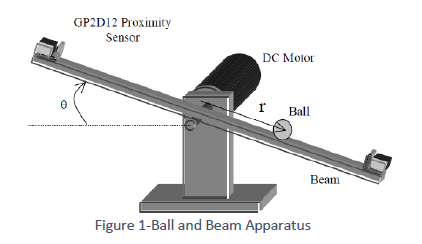
\includegraphics[scale=0.8]{../figures/ballAndBeam.png}
\caption{The ball and beam experiment setup and the system variables $\theta$ and $r$.}
\label{fig:ballAndBeam}
\end{figure}

\begin{table}[h!]
\centering
 \begin{tabular}{||c c c||} 
 \hline
 Abbreviation & Description & Value \\ [0.5ex] 
 \hline\hline
 $m$ & mass of the ball & 0.11 kg \\ 
 $R$ & radius of the ball & 0.015 m \\
 $M$ & mass of the beam & 1 kg \\
 $g$ & gravitational acceleration & 9.8 m/s\textsuperscript{2} \\
 $L$ & length of the beam & 1.0 m \\
 $J_R$ & ball's moment of inertia & 1e-5 kgm\textsuperscript{2} \\
 $J$ & beam's moment of inertia & 2e-3 kgm\textsuperscript{2} \\
 $r$ & ball position coordinate & \\
 $\theta$ & beam angle coordinate &  \\ [1ex] 
 \hline
 \end{tabular}
 \caption{The quantities of the ball and beam system used in the exercise.}
 \label{tab:quantities}
\end{table}

Please note that throughout this report radians have been used for measuring angle.
This means that any reference for $\theta$ has radians as units and any reference to $\dot{\theta}$ has radians per second as unit.
This despite the laboratory instruction refer to degree as the angle unit, values have been converted where relevant. 

\section{Theory}
State space systems are a common way to represent dynamic systems.
For a linear state space system (\ref{equ:genSS}), the time domain solution has been proven to be (\ref{equ:ssSolution}) \citep[~p.189]{astrom21}.

\begin{equation}
\begin{split}
\dot{\textbf{x}} &= A\textbf{x} + B\textbf{u} \\
\textbf{y} &= C\textbf{x}
\end{split}
\label{equ:genSS}
\end{equation}

\begin{equation}
\textbf{y}(t) = Ce^{At}\textbf{x}_0 + C \int_{0}^{t} e^{A(t-\tau)}Bu(\tau) \,d\tau
\label{equ:ssSolution}
\end{equation}

Observability of a system loosely indicates if the system states can be reconstructed from the output. If a system is observable the observer poles can be placed arbitrarily.
The observability matrix is defined \citep[p.~45]{glad00}:

\begin{equation}
\mathcal{O}(A,C) = 
\begin{pmatrix}
C \\ CA \\ \vdots \\ CA^{n-1}
\end{pmatrix}
\label{equ:obsv}
\end{equation}

If the observability matrix $\mathcal{O}$ has full rank (independent rows/columns) the system is observable.

In a similar fashion, controllability loosely indicates if all states of a system can be controlled by the input. If a system is controllable the poles of a state feedback controller can be arbitrarily chosen.
The Controllability matrix is defined \citep[p.~45]{glad00}:

\begin{equation}
\mathcal{S}(A,B) = 
\begin{pmatrix}
B & AB & \cdots & A^{n-1}C
\end{pmatrix}
\label{equ:ctrb}
\end{equation}

If the controllability matrix $\mathcal{S}$ has full rank (independent rows/columns) the system is controllable.

\section{Method}
This section will go though the methodology used to solve the tasks in the order they are assigned in the instructions.
First the system will be modeled and linearized, the modeled system will be analyzed by step and sinusoidal response
Then a controller will be developed based on pole placement and one using optimal control, these will be compared.

\subsection{Modeling and simulation}
This part focus on the derivation of the differential equations governing the ball and beam system.
This is done using Lagrangian Mechanics, a subject not that familiar to the authors of this report.
Due to that limitation and the textbook used for this class not covering the subject help as been taken from \citep{BolvarVincenty2014ModellingTB}.
However several errors have been found in that report, hence it has only been used as inspiration rather than replicating the exact mathematics.

\subsubsection{Equilibrium}
Due to gravity being the force moving the ball, the beam is required to be perpendicular to gravity in order for the ball to be stationary $\theta_0 = 0$.
However the ball can have any position $r_0$ on the perpendicular beam as long as the motor torque $\tau$ cancel the torque on the beam by the ball.
Obviously both derivatives are required to be zero for it to be a stationary point.

\begin{equation}
\textbf{x}_0 = 
\begin{pmatrix}
r_0 \\ \dot{r}_0 \\ \theta_0 \\ \dot{\theta}_0
\end{pmatrix} = 
\begin{pmatrix}
r_0 \\ 0 \\ 0 \\ 0
\end{pmatrix}
\label{equ:stateEqulibrium}
\end{equation}

Where $r_0$ can take any value within the length of the beam $-0.5 < r_0 < 0.5$.

\subsubsection{Selecting variables}
We choose a Cartesian coordinate system centered at the beam pivot point, with $x$ pointing in the direction of $r$ and $y$ pointing up.
The movement of the system can be expressed completely by two independent generalized variables, in our case the ones seen in figure \ref{fig:ballAndBeam}, $r$ and $\theta$.
The relation between the generalized coordinates and the Cartesian coordinates is described below.

\begin{equation}
\begin{split}
x &= r\cos{\theta} \\
y &= -rsin{\theta}
\end{split}
\end{equation}

\subsubsection{Kinetic and Potential energy}
The beam has only rotational kinetic energy $K_1$ and no linear kinetic energy as it is fixed at the pivot point.

\begin{equation}
K_1 = \frac{J\dot{\theta}^2}{2}
\end{equation}

Additionally due to the fixed pivot point, and the origin having been chosen to be that point, the beam has no potential energy.

The ball have both rotational $K_2$ and linear $K_3$ kinetic energy.
The rotational kinetic energy is based on the balls angular velocity $\dot{\theta}_b$ around its rotation point (center).
This rotation occur due to the "no-slip" condition on the contact between the beam and the ball, where the ball has to rotate in order to  move along the beam.

\begin{equation}
K_2 = \frac{J_R\dot{\theta}_b^2}{2} = \frac{J_R\dot{r}^2}{2R^2}
\end{equation}

The linear kinetic energy $K_3$ based on the balls linear velocity $v_b$ can be seen as a combination of the balls radial velocity along the beam and the tangential velocity with the beam.

\begin{equation}
K_3 = \frac{mv_b^2}{2} = \frac{m}{2}(\dot{r}^2 + r^2\dot{\theta}^2)
\end{equation}

The ball also has potential energy $U$ based on the position relative the chosen origin.
Only the direction parallel to gravity (y distance) introduce potential energy.

\begin{equation}
U = mgy = -mgr\sin{\theta}
\end{equation}

Now the total kinetic energy $K$ and total potential energy $U$ can be summarized.

\begin{equation}
\begin{split}
K &= K_1 + K_2 + K_3 = 
\frac{J\dot{\theta}^2}{2} + 
\frac{J_R\dot{r}^2}{2R^2} + 
\frac{m}{2}(\dot{r}^2 + r^2\dot{\theta}^2) \\
&= \frac{J}{2}\dot{\theta}^2 + 
(\frac{J_R}{2R^2} + \frac{m}{2})\dot{r}^2 + 
\frac{m}{2}r^2\dot{\theta}^2 \\
U &= -mgr\sin{\theta}
\end{split}
\end{equation}

\subsubsection{Dynamic system}
With the kinetic and potential energy available from the previous part, the Langrangian $L$ can be setup.

\begin{equation}
L = K - U = 
\frac{J}{2}\dot{\theta}^2 + 
(\frac{J_R}{2R^2} + \frac{m}{2})\dot{r}^2 + 
\frac{m}{2}r^2\dot{\theta}^2 +
mgr\sin{\theta}
\end{equation}

Now the equation of motion for the ball can be calculated using the first Lagrange equation.

\begin{equation}
\begin{split}
\frac{d}{dt}\left(\frac{\partial L}{\partial \dot{r}}\right) - \frac{\partial L}{\partial r} &= 0 \leftrightarrow \\
\frac{d}{dt}\left(\left(\frac{J_R}{R^2} + m\right)\dot{r}\right) - mr\dot{\theta}^2 - mg\sin{\theta} &= 0 \leftrightarrow \\
\left(\frac{J_R}{R^2} + m\right)\ddot{r} - mr\dot{\theta}^2 - mg\sin{\theta} &= 0
\label{equ:ballDiff}
\end{split}
\end{equation}

The right hand side is zero since there are no unaccounted internal or external forces acting on the ball.
Similarly the second Lagrange equation can be used to find the equation of motion for the beam.

\begin{equation}
\begin{split}
\frac{d}{dt}\left(\frac{\partial L}{\partial \dot{\theta}}\right) - \frac{\partial L}{\partial \theta} &= \tau \leftrightarrow \\
\frac{d}{dt}\left(J\dot{\theta} + mr^2\dot{\theta}\right) - mgr\cos{\theta} &= \tau \leftrightarrow \\
(J + mr^2)\ddot{\theta} + 2mr\dot{r}\dot{\theta} - mgr\cos{\theta} &= \tau
\end{split}
\label{equ:beamDiff}
\end{equation}

This time the right hand side is the torque that can be applied to the beam.
The two differential equations (\ref{equ:ballDiff}) and \ref{equ:beamDiff} are the systems governing equations and together describe the system motion.

\begin{equation}
\begin{split}
\begin{cases}
\left(\frac{J_R}{R^2} + m\right)\ddot{r} - mr\dot{\theta}^2 - mg\sin{\theta} = 0 \\
(J + mr^2)\ddot{\theta} + 2mr\dot{r}\dot{\theta} - mgr\cos{\theta} = \tau
\end{cases}
\end{split}
\label{equ:nonLinearDiff}
\end{equation}

\subsubsection{Linearization}
The differential equations (\ref{equ:nonLinearDiff}) obtained with the Lagrange method can be setup as a non linear state space model.

\begin{equation}
\dot{\textbf{x}} = 
\begin{pmatrix}
\dot{x_1} \\ \dot{x_2} \\ \dot{x_3} \\ \dot{x_4}
\end{pmatrix} = 
\begin{pmatrix}
\dot{r} \\ \ddot{r} \\ \dot{\theta} \\ \ddot{\theta}
\end{pmatrix} = 
\begin{pmatrix}
x_2 \\ 
\frac{mx_1x_4^2 + mg\sin{x_3}}{J_R/R^2 + m} \\ 
x_4 \\ 
\frac{- 2mx_1x_2x_4 + mgx_1\cos{x_3} + \tau}{J + mx_1^2}
\end{pmatrix} = f(\textbf{x}, \tau)
\label{equ:nonLinSs}
\end{equation}

To linearize this system the Jacobian $J$ shall be calculated with respect to the state vector $\textbf{x}$ and with respect to the input $\tau$.

\begin{equation}
\begin{split}
\frac{\partial}{\partial \textbf{x}}f(\textbf{x}, \tau) = 
\begin{pmatrix}
0 & 1 & 0 & 0 \\
\frac{mx_4^2}{J_R/R^2 + m} & 0 & \frac{mg\cos{x_3}}{J_R/R^2 + m} & \frac{2mx_1x_4}{J_R/R^2 + m} \\
0 & 0 & 0 & 1 \\
\frac{\partial f_4}{\partial x_1} & -\frac{2mx_1x_4}{J + mx_1^2} & -\frac{mgx_1\sin{x_3}}{J + mx_1^2} & -\frac{2mx_1x_2}{J + mx_1^2}
\end{pmatrix} \\
\frac{\partial f_4}{\partial x_1} = \frac{(-2mx_2x_4 + mg\cos{x_3})(J + mx_1^2) + (-2mx_1x_2x_4 + mgx_1\cos{x_3} + \tau)2mx_1}{(J + mx_1^2)^2}
\end{split}
\label{stateJacobian}
\end{equation}

\begin{equation}
\frac{\partial}{\partial \tau}f(\textbf{x}, \tau) = 
\begin{pmatrix}
0 \\ 0 \\ 0 \\ \frac{1}{J + mx_1^2}
\end{pmatrix}
\label{equ:inputJacobian}
\end{equation}

The linearization will be done around the equilibrium point $\textbf{x}_0$ stated in (\ref{equ:stateEqulibrium}).
For the equilibrium point, the torque $\tau_0$ shall be calculated using $f(\textbf{x}, \tau) = \textbf{0}$.

\begin{equation}
\begin{split}
\frac{-2mx_1x_2x_4 + mgx_1\cos{x_3} + \tau}{J + mx_1^2} &= 0 \rightarrow \\
\frac{mgr_0 + \tau_0}{J + mr_0^2} &= 0 \rightarrow \\
\tau_0 &= -mgr_0
\end{split}
\end{equation}

Now the linearized system can be acquired by populating the Jacobians with the values of the equilibrium point $(\textbf{x}_0, \tau_0)$.

\begin{equation}
\begin{split}
A &= \frac{\partial}{\partial \textbf{x}}f(\textbf{x}_0, \tau_0) = 
\begin{pmatrix}
0 & 1 & 0 & 0 \\
0 & 0 & \frac{mg}{J_R/R^2 + m} & 0 \\
0 & 0 & 0 & 1 \\
\frac{mg}{J + mr_0^2} & 0 & 0 & 0
\end{pmatrix} \\
B &= \frac{\partial}{\partial \tau}f(\textbf{x}_0, \tau_0) = 
\begin{pmatrix}
0 \\ 0 \\ 0 \\ \frac{1}{J + mr_0^2}
\end{pmatrix}
\end{split}
\end{equation}

The linearized system has been included in the result section as (\ref{equ:linSys}).
It has been given a sensor for ball position and beam angle $y = \begin{pmatrix} x_1 & x_3 \end{pmatrix}^T$.

\subsubsection{System simulation}
The instructions ask to simulate the step response of the nonlinear system using the state space equations in (\ref{equ:nonLinSs}).
In order to do this the nonlinear system has to be implemented in in a simulation environment.
To our knowledge, it is not possible to easily simulate nonlinear systems in Matlab, hence the usage of Simulink is motivated.
The nonlinear equations of (\ref{equ:nonLinSs}) are implemented in Simulink along with the constraints mentioned in the instructions, see figure \ref{fig:ballBeamSimulink}.

\begin{figure}[h!]
\center
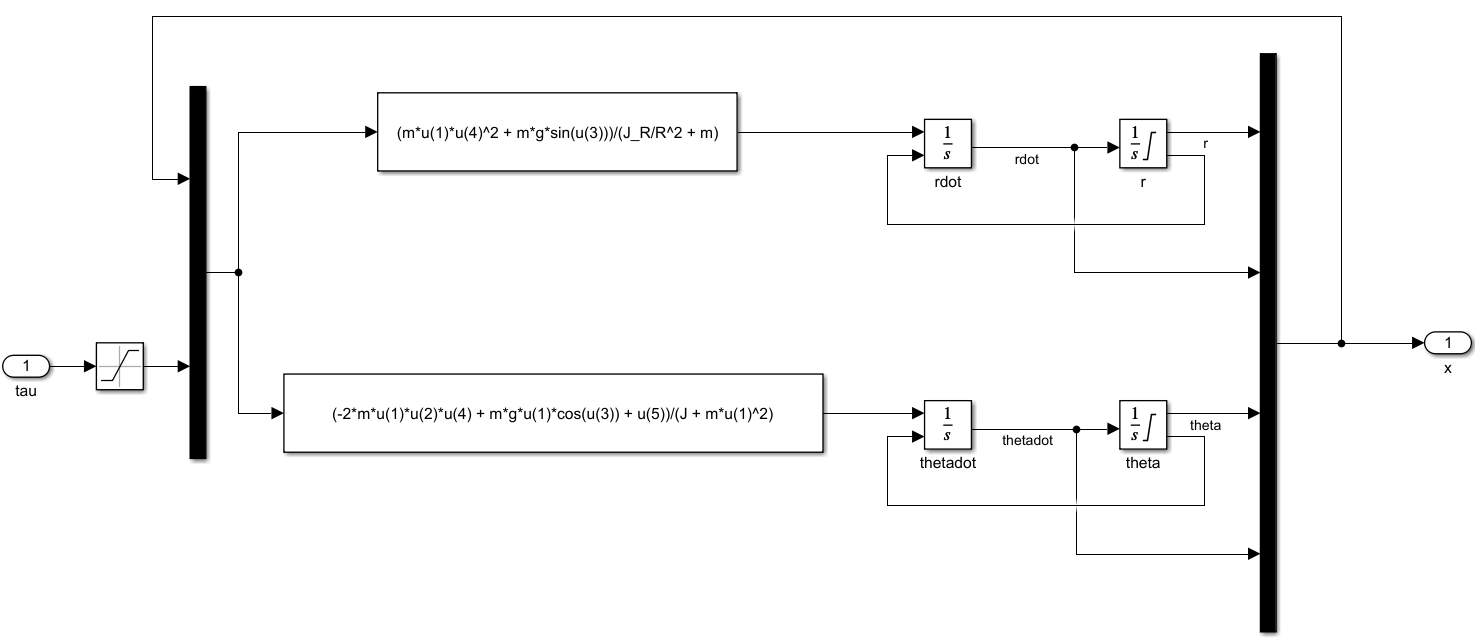
\includegraphics[scale=0.4]{../figures/ballBeamSimulink.png}
\caption{Simulink implementation of ball and beam experiment.}
\label{fig:ballBeamSimulink}
\end{figure}

Setting initial conditions to $\textbf{x}_0 = \begin{pmatrix} 0 & 0 & 0 & 0 \end{pmatrix}^T$, the nonlinear system can be evaluated by both step response and sin wave response.
The step response for the system for a step of size $0.1$ can be seen in results, figure \ref{fig:bbStep}	.
Additionally, attempts were made to "stabilize" the ball on the beam with sine wave stimulation.
A sine wave $\tau = 0.2sin(200\pi t + \pi/2)$ was found to be able to hold the ball on the beam for more than a second.
No sine wave was found that could hold the ball on the beam indefinitely. 
The best resulting sine wave stimulation can be seen in results, figure \ref{fig:sineWave}.
For the sine wave experiment it was found that using an initial condition $\textbf{x}_0 = \begin{pmatrix} 0 & 0 & -2.5e-4 & 0 \end{pmatrix}^T$ aided in keeping the ball centered on the beam.

\subsection{Controller design}
This part focusing on controller design for the ball and beam system modeled and evaluated in the previous section.

\subsubsection{Linear system zero input response}
The equivalent transfer function to the state space system in (\ref{equ:linSys}) can be found using the Matlab command \verb|tf(sys)|.
However, for us to calculate the time domain solution to the system for the initial condition $\textbf{x}_0 = \begin{pmatrix} 0.2 & 0.05 & 1 & 0.01	 \end{pmatrix}^T$ the transfer function is not required.
The first order differential equation system has the solution (\ref{equ:ssSolution}) based on the matrix exponential.
For the zero response, the second part of (\ref{equ:ssSolution}) can be omitted and the solution is:

\begin{equation}
\textbf{y}(t) = Ce^{At}\textbf{x}_0
\end{equation}

Since the system is unstable the solution is expected to grow to infinity as time goes to infinity.
An alternative to calculating solution is to simulate the linear system using the Matlab command \verb|lsim(sys, u, t, x_0)|.
This has been done with the same initial conditions.
For comparison between explicit calculation and simulation see results, figure \ref{fig:zeroIn}.
This figure show the difference between the two solutions.
For both calculation and simulation the system was linearized around the equilibrium $\textbf{x}_0 = \begin{pmatrix} 0 & 0 & 0 & 0 \end{pmatrix}^T$ as it was expected to have zero input (this is the only equilibrium with zero input).

\subsubsection{Controllability and Observability}
Checking both controllability and observability require substantial matrix multiplication for complex systems according to the theory of (\ref{equ:ctrb}) and (\ref{equ:obsv}).
Luckily Matlab offers these operations with implemented function commands \verb|obsv| and \verb|ctrb| along with a check of rank \verb|rank|.
Using these, controllability can be checked easily and all the requested combinations of C matrices can be checked for observability.
Please note that the numerical solution requires numerical matrices for $a, B \& C$, hence the frequently used equilibrium $\textbf{x}_0 = \begin{pmatrix} 0 & 0 & 0 & 0 \end{pmatrix}^T$ has been used.
The result is that the system is controllable and all cases $i - vi$ are observable

\subsubsection{Controller design by pole placement}
In the next sections feedback controllers are designed.
In order to limit the scope of the lab, it is assumed that all the states can be measured.
This reduces to problem to not require an observer.

\begin{equation}
C = \begin{pmatrix}
1 & 0 & 0 & 0 \\
0 & 1 & 0 & 0 \\
0 & 0 & 1 & 0 \\
0 & 0 & 0 & 1 \\ 
\end{pmatrix}
\end{equation}

This allow a state feedback control on the form (\ref{equ:controller}) to be implemented directly on the output $y$.

\begin{equation}
u(t) = -L\textbf{x}(t) + L_r\textbf{r}(t)
\label{equ:controller}
\end{equation}

The gain of $L$ can be found using Matlab built in function \verb|place(sys, p)|.
This function generates the required feedback gains $L$ to have closed-loop poles $p$.
Then the DC gain can be normalized with the reference feed-forward controller.

\begin{equation}
L_r = (C(-A + BL)^{-1}B)^{\dagger}
\label{equ:prefilter}
\end{equation}

Where the $\dagger$ symbol refers to pseudo-inverse.
The assignment then ask to place the poles in $\begin{pmatrix} -7 & -7 & 0.5+0.5i & 0.5-0.5i \end{pmatrix}$, but since this is an unstable set, the system will not respond in a stable manner.
Instead the poles have been placed through purposeful trial and error to try and accommodate the step response specifications of maximum 20\% overshoot and 3s settling time.
The closed-loop poles $\begin{pmatrix} -7 & -6 & -3+3i & -3-3i \end{pmatrix}$ have been found to generate a good step response on the linearized system.
The controller with those poles are now tested with an initial condition of $\textbf{x}_0 = \begin{pmatrix} 0.4 & 0.2 & 0.0175 & 0.0052 \end{pmatrix}^T$ and a reference of zero.
The result with the linearized system can be seen in figure \ref{fig:poleLin} and the result with the nonlinear equations can be seen in figure \ref{fig:poleNon}.
To test the results on the nonlinear system a feedback system was built in Simulink utilizing the ball and beam model from figure \ref{fig:ballBeamSimulink}.
It utilizes the standard state feedback controller form for $L$ with a prefilter $L_r$ on the reference input, see figure \ref{fig:feedbackSys}.

\begin{figure}[h!]
\center
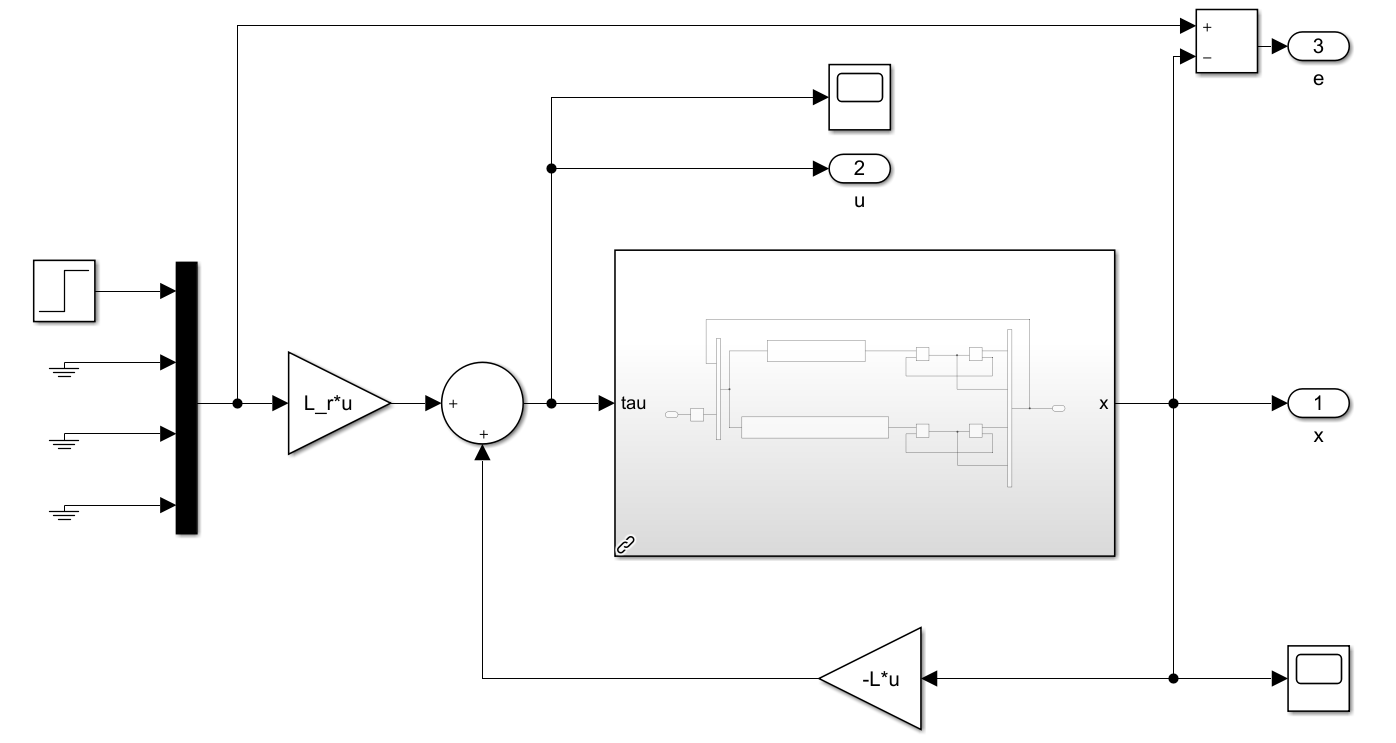
\includegraphics[scale=0.4]{../figures/feedbackSystemSimulink.png}
\caption{Simulink implementation of state feedback for the nonlinear ball and beam implementation. The step input here has mainly been used for testing purposes while the results in the report use a zero reference for all states.}
\label{fig:feedbackSys}
\end{figure}

\subsubsection{Optimal controller design}
Optimal control is achieved by minimizing a cost function:

\begin{equation}
J = \int_0^{\infty} \Delta \textbf{x}^TQ\Delta \textbf{x} + \Delta u^TR\Delta u\,dt
\end{equation}

The controller on the same form as before (\ref{equ:controller}) that minimizes the cost function can be found using the built-in Matlab function \verb|lqr(sys, Q, R)|.
Then the prefilter for unity DC gain $L_r$ can be calculated just as before (\ref{equ:prefilter}) as well.
The operation start by using an identity matrix for $Q$ and $1$ for $R$, then by purpose full trial and error weights that generate good results where found.
The resulting weights that was found are:

\begin{equation}
Q = \begin{pmatrix}
30 & 0 & 0 & 0 \\
0 & 1 & 0 & 0 \\
0 & 0 & 1 & 0 \\
0 & 0 & 0 & 1
\end{pmatrix}, \; 
R = 1
\end{equation}

The performance results of the optimal controller for the same initial conditions as before and a return to zero step can be seen in results, figure \ref{fig:lqrLin} for the linearized system and figure \ref{fig:lqrNon} for the nonlinear ball and beam.

\subsubsection{Controller comparison}
The pole placement method and the optimal control approach used in previous sections are now compared.
They are compared using the norms of the error signal and the control signal, taking advantage of the Matlab function \verb|norm|.
The norm of the error signal is calculated over full state vector error to incorporate the whole system divergence from the reference.
Additionally they are compared using overshoot, calculated on only the ball position value $r$.
Also the settling time of the ball position is compared for a settling within $\pm5\%$.
The calculated comparison result can be found under results, table \ref{tab:compare}.





\section{Results}
This section list the results acquired during the laboratory work.

\subsection{Linearized system}
The linearized system for the ball and beam is presented below for an equilibrium point $\textbf{x}_0 = \begin{pmatrix} r_0 & 0 & 0 & 0 \end{pmatrix}^T$, $\tau_0 = -mgr_0$.

\begin{equation}
\begin{split}
\dot{\Delta\textbf{x}} &= 
\begin{pmatrix}
0 & 1 & 0 & 0 \\
0 & 0 & \frac{mg}{J_R/R^2 + m} & 0 \\
0 & 0 & 0 & 1 \\
\frac{mg}{J + mr_0^2} & 0 & 0 & 0
\end{pmatrix}\Delta\textbf{x} + \begin{pmatrix}
0 \\ 0 \\ 0 \\ \frac{1}{J + mr_0^2}
\end{pmatrix}\Delta\tau \\
\Delta y &= \begin{pmatrix}
1 & 0 & 0 & 0 \\
1 & 0 & 1 & 0
\end{pmatrix}\Delta\textbf{x}
\end{split}
\label{equ:linSys}
\end{equation}


\subsection{System simulation}
Simulating the nonlinear equations in (\ref{equ:nonLinSs}) and their response to a step input and sine wave input can be seen in figure \ref{fig:bbStep} and \ref{fig:sineWave} respectively.

\begin{figure}[H]
\center
\includegraphics[scale=0.75]{../code/figures/bbStep.png}
\caption{Ball and beam step response to a torque step of 0.1Nm at 0.1s.}
\label{fig:bbStep}
\end{figure}

\begin{figure}[H]
\center
\includegraphics[scale=0.75]{../code/figures/sineWave.png}
\caption{Ball and beam sine wave response to a sine wave of amplitude 0.2Nm and frequency 100Hz. The sine wave has been made to attempt to hold the ball on the beam for as long as possible.}
\label{fig:sineWave}
\end{figure}

\subsection{Linear system zero input response}
The time evolution of the linearized system (\ref{equ:linSys}) grows to infinity for the initial condition $\textbf{x}_0 = \begin{pmatrix} 0.2 & 0.05 & 1 & 0.01 \end{pmatrix}^T$.
This solution has been calculated explicitly and by simulation and the difference between the results can be seen in figure \ref{fig:zeroIn}.

\begin{figure}[H]
\center
\includegraphics[scale=0.75]{../code/figures/zeroIn.png}
\caption{Difference between the explicit solution and the simulated solution for the linearized ball and beam system}
\label{fig:zeroIn}
\end{figure}

\subsection{Controllability and Observability}
The linearized system (\ref{equ:linSys}) is controllable.
The system is also observable for all cases $i - vi$ of $y$.

\subsection{Controller design by pole placement}
The state feedback controller that was designed using pole placement with poles at  $\begin{pmatrix} -7 & -6 & -3+3i & -3-3i \end{pmatrix}$ gave performance on the linearized system seen in figure \ref{fig:poleLin}.
The performance of the same controller on the nonlinear ball and beam equations can be seen in figure \ref{fig:poleNon}.
The evaluation was done checking the return to zero response of the system with an initial condition of $\textbf{x}_0 = \begin{pmatrix} 0.4 & 0.2 & 0.0175 & 0.0052 \end{pmatrix}^T$.

\begin{figure}[H]
\center
\includegraphics[scale=0.75]{../code/figures/figPoleLin.png}
\caption{Linearized system response with a state feedback controller designed to have closed-loop poles in $\begin{pmatrix} -7 & -6 & -3+3i & -3-3i \end{pmatrix}$.}
\label{fig:poleLin}
\end{figure}

\begin{figure}[H]
\center
\includegraphics[scale=0.75]{../code/figures/figPoleNon.png}
\caption{Nonlinear ball and beam system response with a state feedback controller designed to have closed-loop poles in $\begin{pmatrix} -7 & -6 & -3+3i & -3-3i \end{pmatrix}$.}
\label{fig:poleNon}
\end{figure}

\subsection{Optimal controller design}
The state feedback controller that was designed using optimal control methods gave performance on the linearized system seen in figure \ref{fig:lqrLin}.
The performance of the same controller on the nonlinear ball and beam equations can be seen in figure \ref{fig:lqrNon}.
The evaluation was done checking the return to zero response of the system with an initial condition of $\textbf{x}_0 = \begin{pmatrix} 0.4 & 0.2 & 0.0175 & 0.0052 \end{pmatrix}^T$.

\begin{figure}[H]
\center
\includegraphics[scale=0.75]{../code/figures/figLqrLin.png}
\caption{Linearized system response with a state feedback controller designed using optimal control techniques.}
\label{fig:lqrLin}
\end{figure}

\begin{figure}[H]
\center
\includegraphics[scale=0.75]{../code/figures/figLqrNon.png}
\caption{Nonlinear ball and beam system response with a state feedback controller designed using optimal control techniques..}
\label{fig:lqrNon}
\end{figure}

\subsection{Controller comparison}
The table \ref{tab:compare} below showcase the performance metrics comparison between the usage of pole placement and optimization for state feedback control.

\begin{table}[h!]
\centering
 \begin{tabular}{||c c c||} 
 \hline
 Metric & Pole placement & Optimization \\ [0.5ex] 
 \hline\hline
 $\left\lVert \textbf{e}(t)\right\rVert_2^2$ & 30.4 & 22.0 \\ 
 $\left\lVert \textbf{e}(t)\right\rVert_\infty$ & 9.1 & 6.6 \\
 $\left\lVert u(t)\right\rVert_2^2$ & 4.1 & 4.8 \\
 $\left\lVert u(t)\right\rVert_\infty$ & 0.55 & 0.99 \\
 overshoot [\%] & 31.8 & 0.0 \\
 settling time [s] & 1.75 & 1.60 \\ [1ex] 
 \hline
 \end{tabular}
 \caption{Comparison of pole placement method and optimal control method performance on a return to zero response for the nonlinear ball and beam.}
 \label{tab:compare}
\end{table}


\section{Discussion}
- White box modeling is difficult
- Linearization is error prone
- Step response = Unstable system, 0.1Nm enough to dominate the ball weights
- Sine wave: Centering the beam oscillations
- Step response of linear and nonlinear similar around [0 0 0 0]

\section{Conclusion}

\clearpage
\bibliography{reference}

\clearpage
\appendix

\section{Example Section}
This is an example reference \citep{glad00}.

\begin{figure}[h!]
\center
\includegraphics[scale=0.8]{../code/figures/exampleFigure.png}
\caption{Example caption.}
\label{fig:exampleLable}
\end{figure}

\lstinputlisting{../code/exampleCode.m}

\end{document}